% (c) Gerard Baecker
\documentclass[fleqn,a4paper,12pt]{article}
\usepackage[german]{babel}
\usepackage[utf8]{inputenc}
%\usepackage{amsmath}    % Mathematische Symbole
\usepackage{amssymb}     % Nochmehr mathematische Symbole
\usepackage{dsfont}      % Schriftsatz fuer Zahlenmengensymbole
%\usepackage{verbatim}   % erweiterte Verbatim-Umgebung
\usepackage{alltt}       % Quasi-Verbatim-Umgebung
\usepackage{fancyhdr}    % Eigene Kopfzeilen
\usepackage{graphicx}    % Zum Einbinden von Grafiken
% Einbinden einer eps-Grafik geht so: includegraphics{path}

% Seitenraender
\addtolength{\voffset}{-2cm}
\addtolength{\textheight}{0cm}
\addtolength{\hoffset}{0cm}
\addtolength{\textwidth}{2cm}
\addtolength{\headheight}{2cm} % fuer jeden Strichkode einen Zentimeter

% Skalierung der Grafiken
\setlength{\unitlength}{1cm}

\pagestyle{fancy}            % Eigene Kopfzeilen verwenden
\frenchspacing               % Kein Extrafreiraum nach Satzzeichen
\setlength{\parindent}{0pt}  % Neue Absaetze nicht einruecken
%\sloppy                     % Schlampige Absatzformatierung
\fussy                       % Penible Absatzformatierung
\linespread{1.5}             % Zeilenabstand

% Font fuer Code 39
\font\xlix=wlc39 scaled 1200
\newcommand\barcode[1]{{\xlix@#1@}}

% Name, Matrikelnummer, Barcode
\newcommand\student[2]{
  \mbox{\scriptsize
  \begin{tabular}{@{}l@{}r@{}}
    \multicolumn{2}{@{}r@{}}{\barcode{#2}}\\
    #1&#2\\
  \end{tabular}}}

% Kopfzeile
\lhead{
  \small
  \textsc{Grundlagen der Signalverarbeitung \\
    WS 2017/2018 \\
    \"Ubung (\today)}
  \vfill}
\rhead{
  \begin{tabular}[b]{@{}rr@{}}
    \student{Philipp Badenhoop}{572693} &
    \student{Steven Lange}{568733} \\
    \student{Pascal Jochmann}{575056} &
    \student{Kevin Trogant}{572451}
  \end{tabular}}

\begin{document}
"Ubungsaufgabe 1: \newline
\begin{itemize}
  \item Raumtemperatur in meinem Zimmer über einen Tag (lässt sich mit Thermometer messen)
  \item Wert meiner Aktien über den Zeitraum eines Monats (lässt sich mit Börsenapps nachverfolgen)
  \item Stromverbrauch (in Watt) der Geräte an einer Steckdose über eine Woche (durch Stromverbrauchmessgerät)
\end{itemize}
\newpage
"Ubungsaufgabe 2:\newline
\begin{figure}
  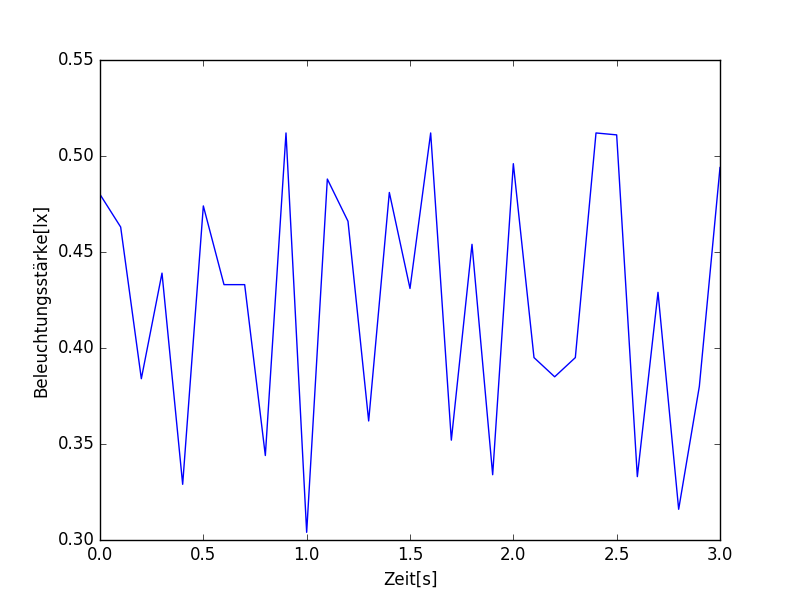
\includegraphics[width=1.0\textwidth]{signal.png}
\end{figure}
Anmerkung: Die Linien, die die Punkte verbinden sind nur zur besseren Übersicht.\newline
Der Prozess ist zufällig, denn es lässt sich keine Periodizität oder Form erkennen, die auf eine typische mathematische Funktion (z.B. Sinus) hindeuten würde.

\end{document}
